\label{subsec:optimization}
Instead of selecting fiducals from one method for all the parts as explained in earlier section,
here we propose a method which selects fiducials for each part from best performing method. 
We first collect fiducials from all the candidate algorithms on an input image. Our task is now to
select a subset of these fiducials for our output. 

We propose an optimization framework based on equation~\ref{eq:main_second_equation},
 where we minimize a function based on appearence and structural
costs. The appearance cost forces the areas around the fiducial locations in the input image 
to ``look'' like a face, while the structural cost ensures that the outline of fiducial locations 
resembles a facial structure. We define a quadratic objective function with unary and binary terms
that enforce these constraints. Unary terms enforce appearance costs, while binary terms enforce
structural costs.

The selection of the $j^{th}$ fiducial from the
$i^{th}$ method is represented by the binary variable $x_i^j$.  Let $u_i^j$ be its
appearence cost. Let $y_{cd}^{ab}$ be the selection variable which will be $1$ when both $x_c^a$
and $x_d^b$ are $1$. And, $p_{cd}^{ab}$ define the structural cost when $y_{cd}^{ab}$ is $1$.
Thus $y^{ab}_{cd}$ is the binary variable that represents \emph{joint selection} of fiducials
corresponding to unary variables $x^a_c$ and $x^b_d$.

\textbf{Appearance Costs:} We would want the fiducial prediction for each part to look similar to the corresponding fiducial  
of \emph{one} of the exemplars. To do this, we compare the appearance feature vectors (using SIFT
and HOG) between the fiducial $x_i^j$ and that of the corresponding fiducials in the exemplar
database.
Let $f(x^j_i)$ represent the appearance feature vector corresponding to the $j^{th}$ fiducial
produced by the $i^{th}$ method. We define the unary costs as
\begin{equation}
  u^j_i = \arg\min_k \Vert f(x^j_i) - f(\mathcal{E}^j_k) \Vert^2
\end{equation}
where $\mathcal{E}^j_k$ denotes the $j^{th}$ part of the $k^{th}$ exemplar. Let $m(j, i)$ represent
the exemplar index that has the fiducial closest in appearance to that of $x^j_i$. That is, 
let $u^j_i = \Vert f(x^j_i) - f(\mathcal{E}^j_{m(j,i)}) \Vert^2$.
% Therefore, we define appearence cost, $u_j^i$ as, $u_j^i = min(appDist_1^j,
% appDist_2^j, \ldots , appDist_N^j)$. Where $appDist_n^j$ is the Euclidean distance between the
% appearence feature vectors at fiducal prediction by method $i$ for part $j$ and at ground truth
% location of exemplar $n$ at part $j$.
\textbf{Structural Costs:} We would also want to preserve the facial structure while selecting fiducials. This is most
naturally enforced in the binary variable cost $p^{ab}_{cd}$. 
The importance of this cost is depicted in Figure~\ref{fig:with_without_structural_costs}.
We enforce structural consistency by ensuring that if
two fiducials $x^a_c$ and $x^b_d$ are selected, their corresponding closest exemplars (given
by indices $m(a,c)$ and $m(b,d)$ as mentioned above) are as close to each other in shape as
possible. Thus, we define the structural cost $p^{ab}_{cd}$ as the euclidean distance between
the shape of exemplars $\mathcal{E}_{m(a,c)}$ and $\mathcal{E}_{m(b,d)}$. Note that the structural
cost is only defined between two variables that \emph{do not} represent the same fiducial. 
That is
\begin{equation}
  p^{ab}_{cd} = \Vert s(\mathcal{E}_{m(a,c)}) - s(\mathcal{E}_{m(b,d)}) \Vert^2, \qquad a \ne b
\end{equation}
where $s(\cdot)$ is the function that denotes the shape of a set of fiducials (represented as a
vector of fiducial locations).
Additionally, we also want to enforce the constraint that the same fiducial from different methods
should not be simultaneously selected. This is easily enforced by the constraint
\begin{equation}
  \sum_i x^j_i = 1
\end{equation}
Combining all the above, we want to minimize the following function function,
\begin{equation}
O(X,Y) = \sum_{i=1}^{5} \sum_{j=1}^{20} (x^j_i \times u_i^j) + \sum_{c=1}^{20} \sum_{d=c+1}^{20} \sum_{a=1}^{5} \sum_{b=1}^{5} (y_{cd}^{ab} \times p_{cd}^{ab})
\end{equation}
subjected to constraints,
$x_i^j \in \{0,1\}$, $y_{cd}^{ab} \in \{0,1\}$, $\sum_{i=1}^5 x_i^j = 1$, $y_{cd}^{ab} = x_c^a \times x_d^b$


%We would also want to preserve the facial structure while selecting landmarks. Since the individual methods already take care of structural constraints, we define structural cost as, $p_{cd}^{ab} = structDist^{ab}$. Where $structDist^{ab}$ is the Euclidean distance between the landmark prediction vectors of method $a$ and $b$. This will ensure the selected landmarks would look like a face.

Since the above problem has quadratic constraints and can not be solved in polynomial time, as the solutions are in integers, we
relax the constraints~\cite{DBLP:journals/corr/ChariLLS14} to get:
$0 \leq x_i^j \leq 1$, $0 \leq y_{cd}^{ab} \leq 1$, $x_c^a \geq y_{cd}^{ab}$, $x_d^b \geq
y_{cd}^{ab}$, $x_c^a + x_d^b \le y_{cd}^{ab} + 1$. Thus, we obtain the final linear
optimization problem as 
\begin{eqnarray}
O(X,Y) & = & \sum_{i=1}^{5} \sum_{j=1}^{20} (x_i^j \times u_i^j) + \nonumber \\
        & & \sum_{c=1}^{20} \sum_{d=c+1}^{20} \sum_{a=1}^{5} \sum_{b=1}^{5} (y_{cd}^{ab} \times p_{cd}^{ab}) \nonumber \\
        & & 0 \leq x_i^j, y^{ab}_{cd} \leq 1, x_c^a \geq y_{cd}^{ab}, x_d^b \geq y_{cd}^{ab} \nonumber \\
        & & x_c^a + x_d^b \le y_{cd}^{ab} + 1 
\end{eqnarray}
We use {\tt MOSEK} wrapper in MATLAB to solve the above optimization problem. Sometimes, because of
the non-linear nature of the problem, we get non-integer solutions for $x^j_i$. In such cases, we
take our fiducial location to be the average position of the top two selected outputs for the
$j^{th}$ part.

\begin{figure}
\centering
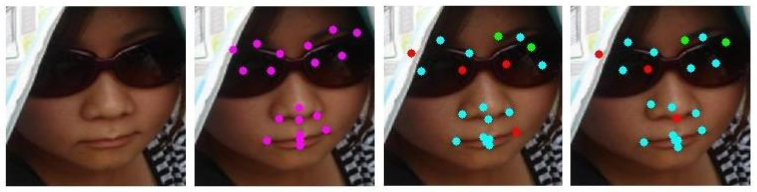
\includegraphics[width=4.5in,height=1.3in]{fid/figures/with_without_pairwise.png}
\caption{From left to right, we observe input test image, output selection by kNN, output selection by optimization without structural costs and output selection by optimization with structural costs. Observe that the left eye prediction suffers in third image because of not considering structural costs for optimization.}
\label{fig:with_without_structural_costs}
\end{figure}

